\secnumbersection{DISEÑO EXPERIMENTAL}
En el presente capítulo, se describen los aspectos generales con respecto al diseño experimental de la memoria, es decir, por una parte se establecen las métricas a utilizar para la evaluación de los algoritmos y como se utilizarán dichas métricas. También se define el flujo de comandos y como se procesa la información desde los sensores, como también se describe el diseño, prototipo y versión física (tanto estructura como componentes electrónicos) del robot utilizado para desarrollar la memoria. Por último, se definen en detalle los ambientes utilizados para la realización de las pruebas.

\subsection{IMPLEMENTACIÓN}
\subsubsection{DISEÑO}
El prototipo del robot fue diseñado en el software de Autodesk, Fusion360 siguiendo los requerimientos, especificaciones y medidas reales. Fue un proceso incremental en dónde se realizaron diversas pruebas y diseños hasta llegar a la versión final utilizada. Consta de una estructura de aluminio donde están montadas las ruedas y motores, sobre dicha estructura con un verde esmeralda está impreso en 3D el cuerpo del robot separado en 4 zonas:
\begin{itemize}
    \item \textbf{Cuerpo: }Estructura que une la base metálica con el resto del cuerpo.
    \begin{figure}[H]
        \centering
        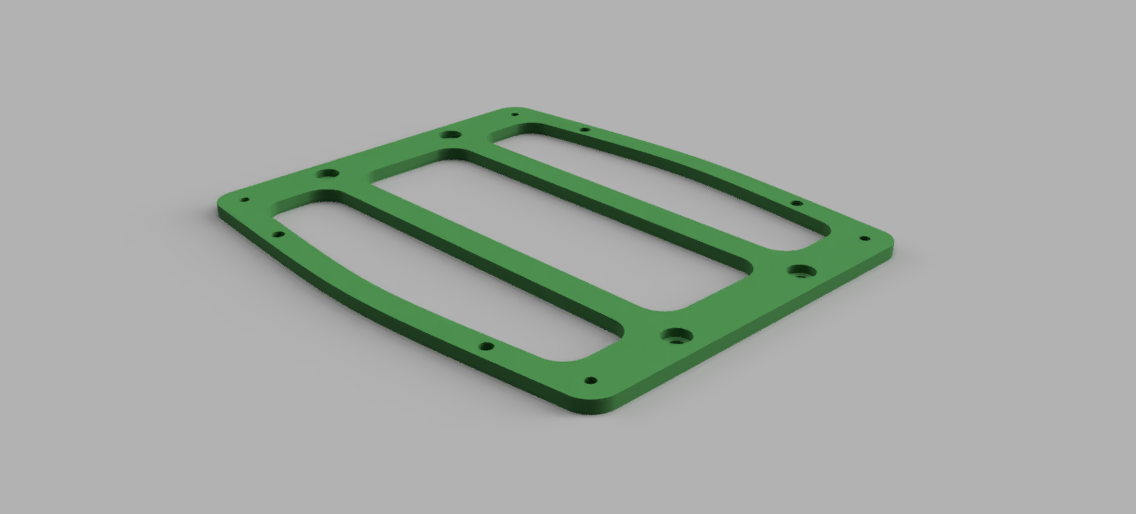
\includegraphics[width=7cm]{figures/04diseño_experimental/base_cuerpo.png}
        \caption{ Diseño del cuerpo del robot } 
        Fuente: Fabricación propia
        \label{fig:robocop_cuerpo}
    \end{figure}
    \item \textbf{Montura cámara: }Estructura frontal donde va montada la cámara de profundidad, dicha estructura va unida al cuerpo.
    \begin{figure}[H]
        \centering
        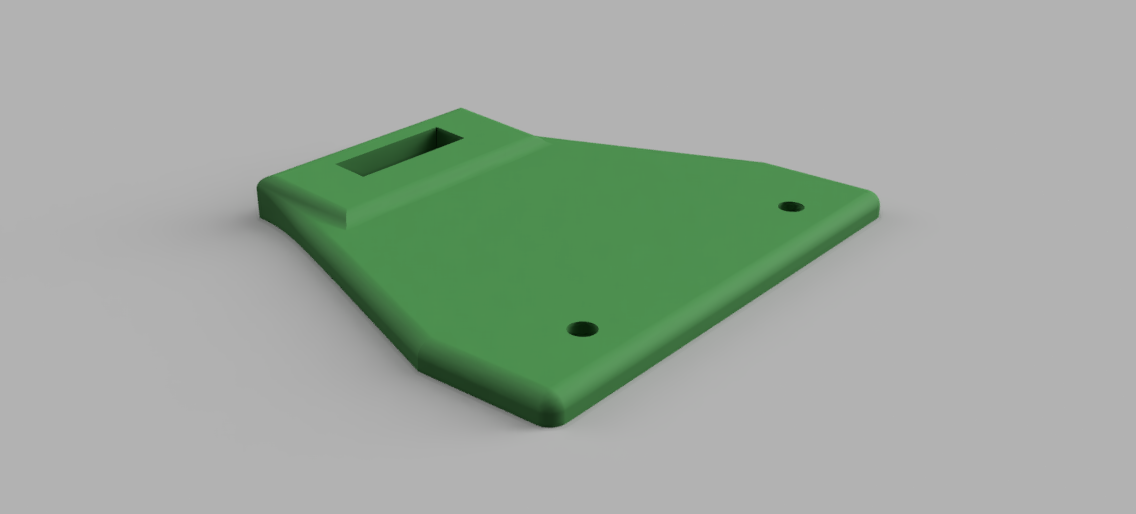
\includegraphics[width=7cm]{figures/04diseño_experimental/soporte_camara.png}
        \caption{ Diseño de la montura de la cámara} 
        Fuente: Fabricación propia
        \label{fig:robocop_camara}
    \end{figure}
    \item \textbf{Montura electrónica: }Estructura central donde va montada toda la electrónica del robot, es decir, el arduino, la orange pi, las baterías y el lidar. Dicha estructura va unida al cuerpo.
    \begin{figure}[H]
        \centering
        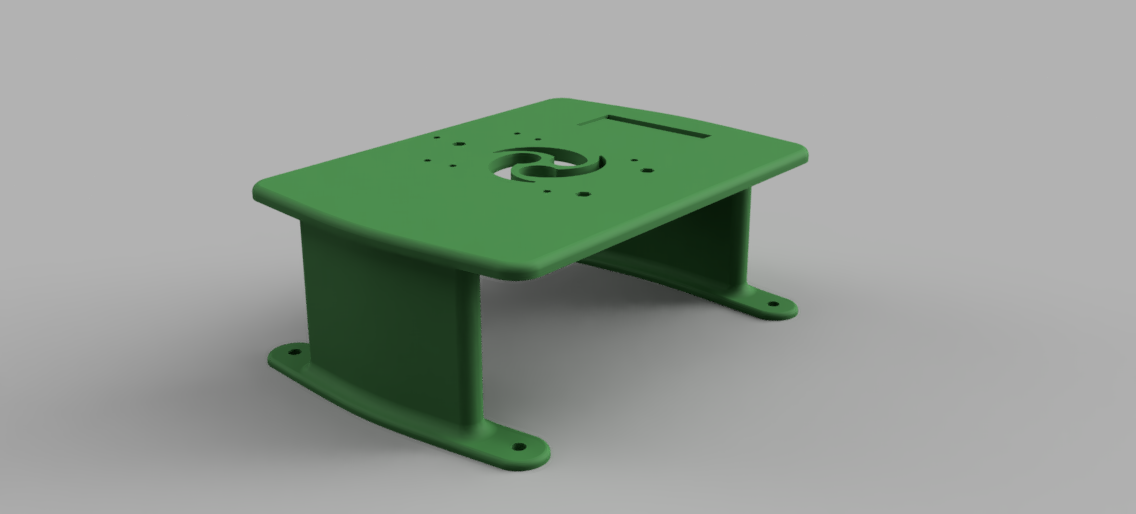
\includegraphics[width=7cm]{figures/04diseño_experimental/soporte_electronica.png}
        \caption{ Diseño de la montura de la electrónica} 
        Fuente: Fabricación propia
        \label{fig:robocop_electronica}
    \end{figure}
    \item \textbf{Montura pantalla: }Estructura posterior donde va montada la pantalla del robot para tener acceso al sistema operativo detrás de este.
    \begin{figure}[H]
        \centering
        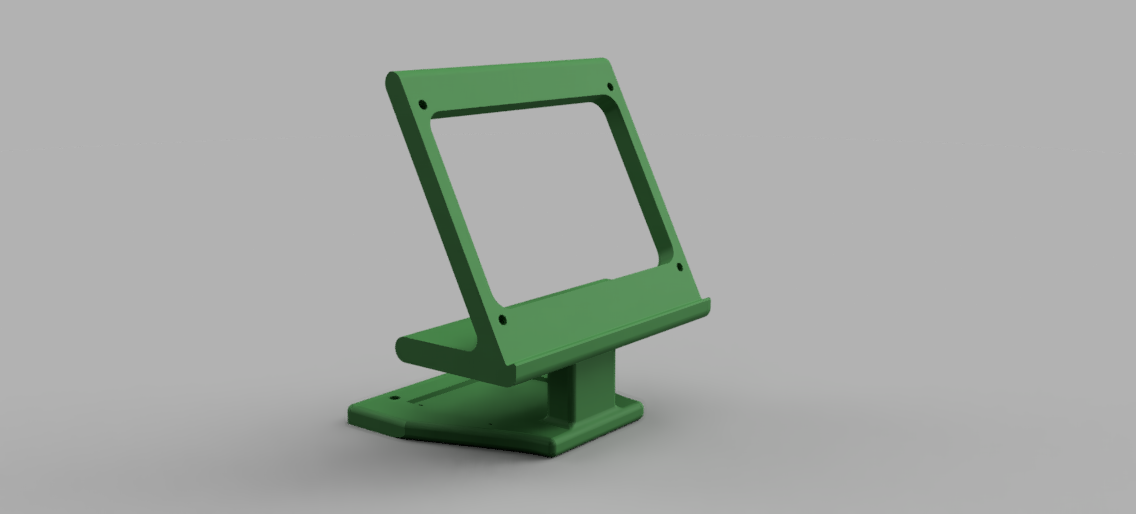
\includegraphics[width=7cm]{figures/04diseño_experimental/soporte_pantalla.png}
        \caption{ Diseño de la montura de la pantalla} 
        Fuente: Fabricación propia
        \label{fig:robocop_pantalla}
    \end{figure}
\end{itemize}

El diseño final, con las piezas montadas y las estructuras ensambladas se puede observar en la Figura  \ref{fig:robocop_diseño}.
\begin{figure}[H]
\centering
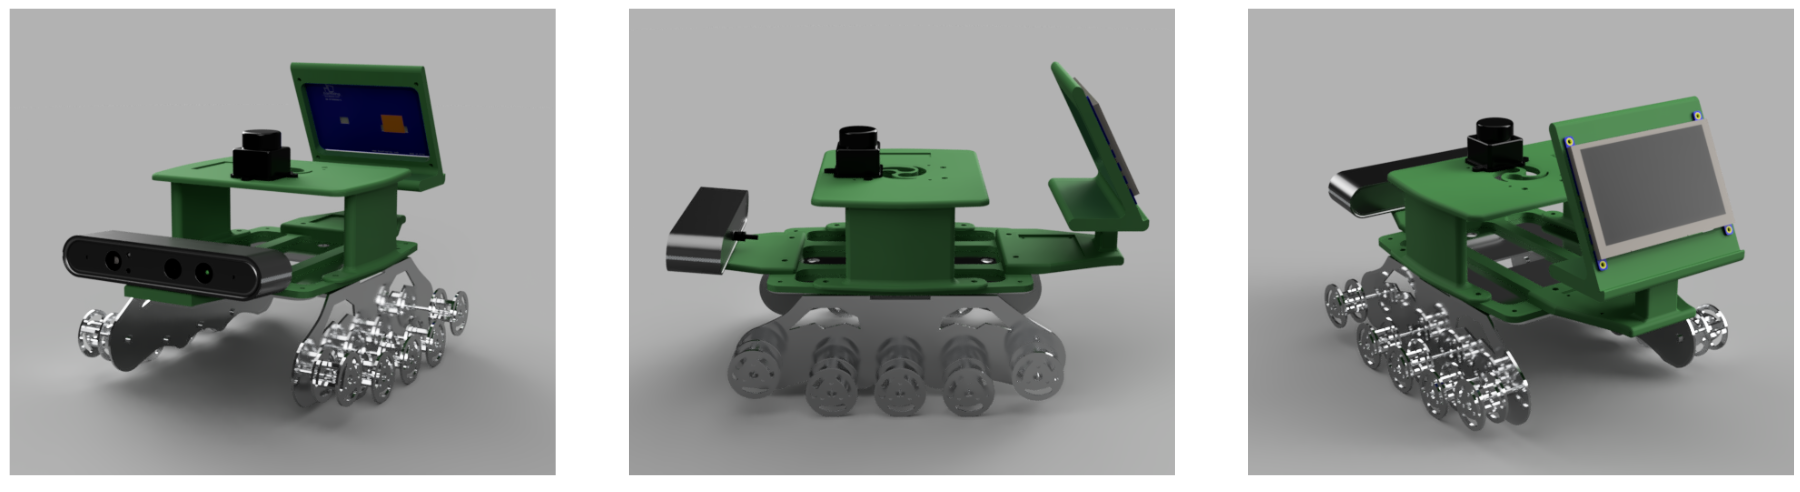
\includegraphics[width=15cm]{figures/04diseño_experimental/robocop_diseño.png}
\caption{ Diseño del robot realizado en Fusion360 } 
Fuente: Fabricación propia
\label{fig:robocop_diseño}
\end{figure}

\subsubsection{SIMULACIÓN}
La simulación tanto del robot como de los algoritmos descritos anteriormente se realizó con el software gazebo, para así probar todos los elementos sin riesgos de dañar los componentes electrónicos. Los resultados de dicha simulación se pueden observar en Figura \ref{fig:robocop_simulado} en dónde se observa el robot simulado correctamente en un ambiente interior.

\begin{figure}[H]
\centering
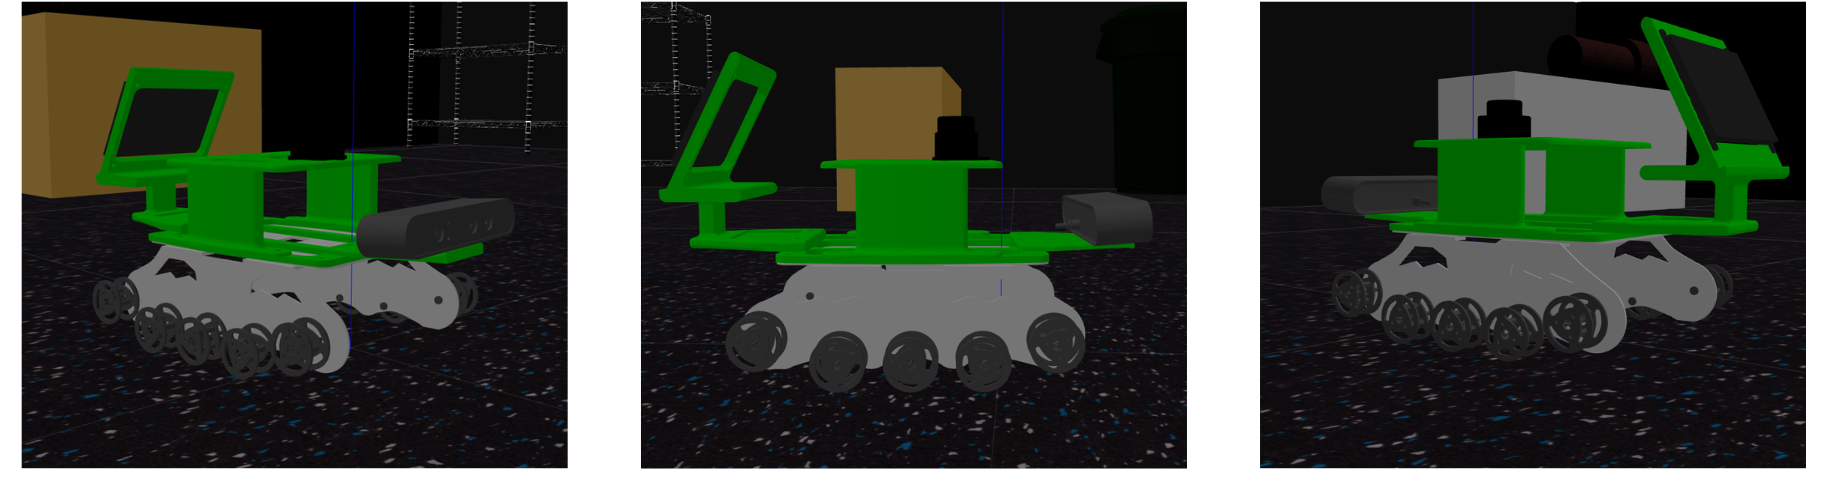
\includegraphics[width=15cm]{figures/04diseño_experimental/robocop_simulado.png}
\caption{Simulación en gazebo del robot diseñado}
Fuente: Fabricación propia
\label{fig:robocop_simulado}
\end{figure}


\newpage
\subsection{ROBOT FÍSICO}
En la presente sección, se describirá en detalles al robot diseñado para la realización de la memoria, se en listarán tanto los sensores utilizados, los componentes electrónicos y el diagrama del flujo de la información y/o comandos. El prototipo real del robot diseño se puede observar en la Figura \ref{fig:robocop_real}, representando de manera correcta lo diseñado, se pueden examinar la posición de los distintos componentes electrónicos, sensores y la estructura final hecha. Para simplicidad del estudio, se construyó un robot diferencial \footnote{Un robot diferencial es aquel robot en que tiene dos pares de ruedas (o grupos de rueda) que son independientes entre sí, es decir, la velocidad de movimiento depende de la diferencia entre el movimiento de estos dos grupos.}, con un volumen de aproximadamente 37 [cm] x 26 [cm] x 26 [cm], dicho volumen será utilizado por los algoritmos para evitar las colisiones al momento de planificar la ruta y realizar la navegación autónoma.

\begin{figure}[H]
\centering
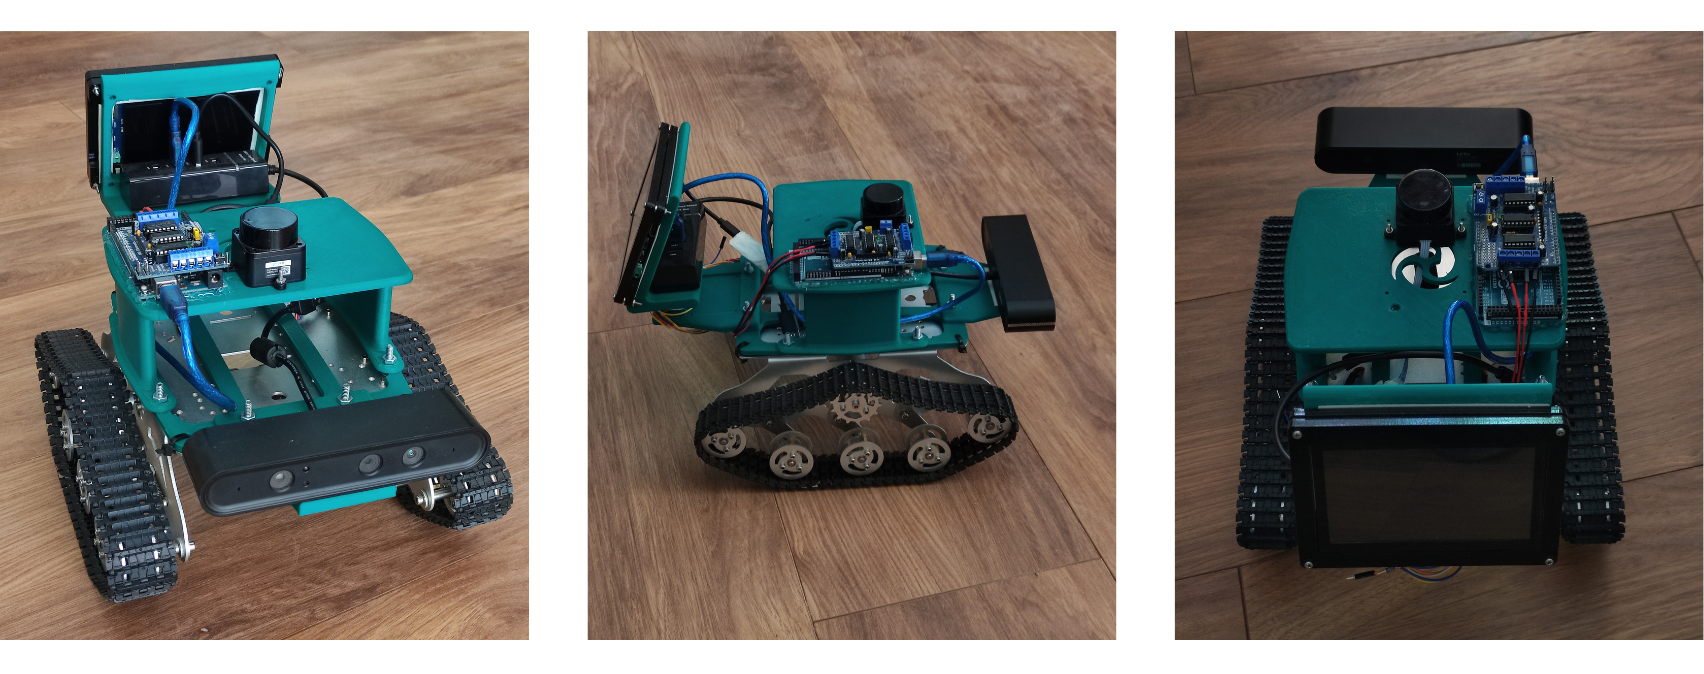
\includegraphics[width=15cm]{figures/04diseño_experimental/RoboCop.png}
\caption{Prototipo real del robot diseñado}
Fuente: Fabricación propia
\label{fig:robocop_real}
\end{figure}

\subsubsection{COMPONENTES ELECTRÓNICOS}
En la Tabla \ref{tab:componentes_electronicos} se pueden observar los componentes electrónicos utilizados para la construcción del robot, tanto su nombre como su imagen asociada. Dentro de los componentes se pueden destacar la \textbf{orange pi}, la cual corresponde al computador principal del robot, la cual realizará todo el procesamiento de los datos, los sensores \textbf{LD19} y \textbf{Orbbec Astra Pro} para escanear y construir los mapas, el \textbf{Arduino Mega} el cual controlará los motores y finalmente el \textbf{Wit motion BWT901BLECL} el cual proporcionará los datos de la velocidad angular, aceleración y orientación.
\begin{table}[H]
    \centering
    \begin{tabular}{|c|c|c|}
    \hline
    \textbf{N°} & \textbf{Nombre}  & \textbf{Imagen} \\ \hline
    \hline
    \textbf{1}  & Orange Pi 4GB RAM  & 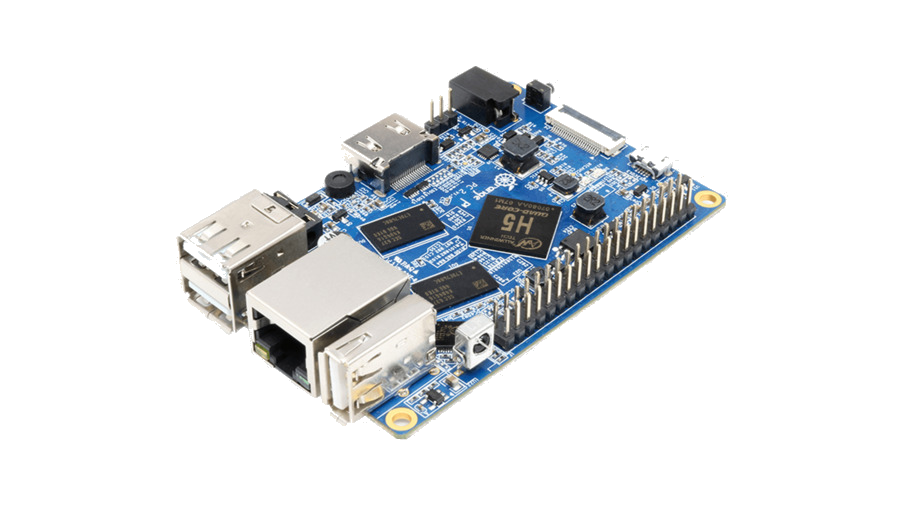
\includegraphics[width=4cm, height=2.3cm]{figures/04diseño_experimental/orange_pi.png} 
    \\ \hline
    \textbf{2}  & Arduino Mega     &  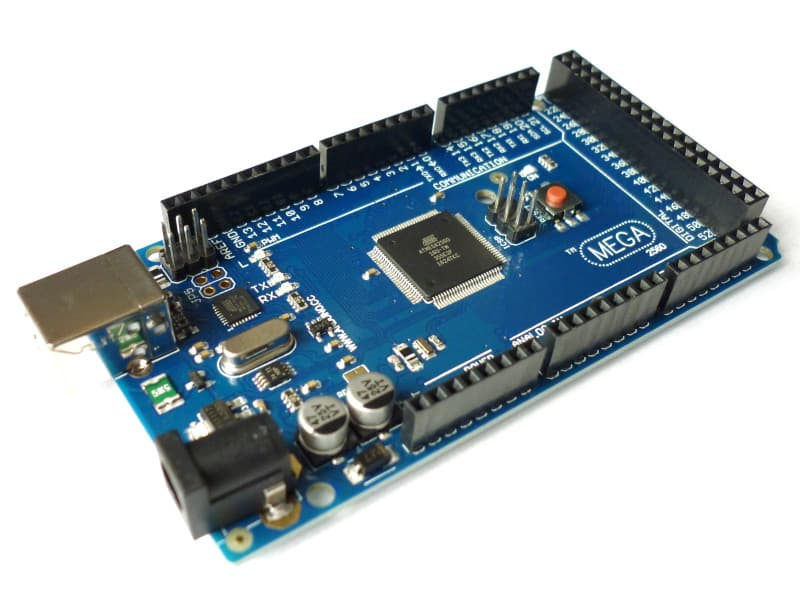
\includegraphics[width=3cm, height=2.3cm]{figures/04diseño_experimental/arduino_mega.jpg}
    \\ \hline
    \textbf{3}  & Shield Puente H  & 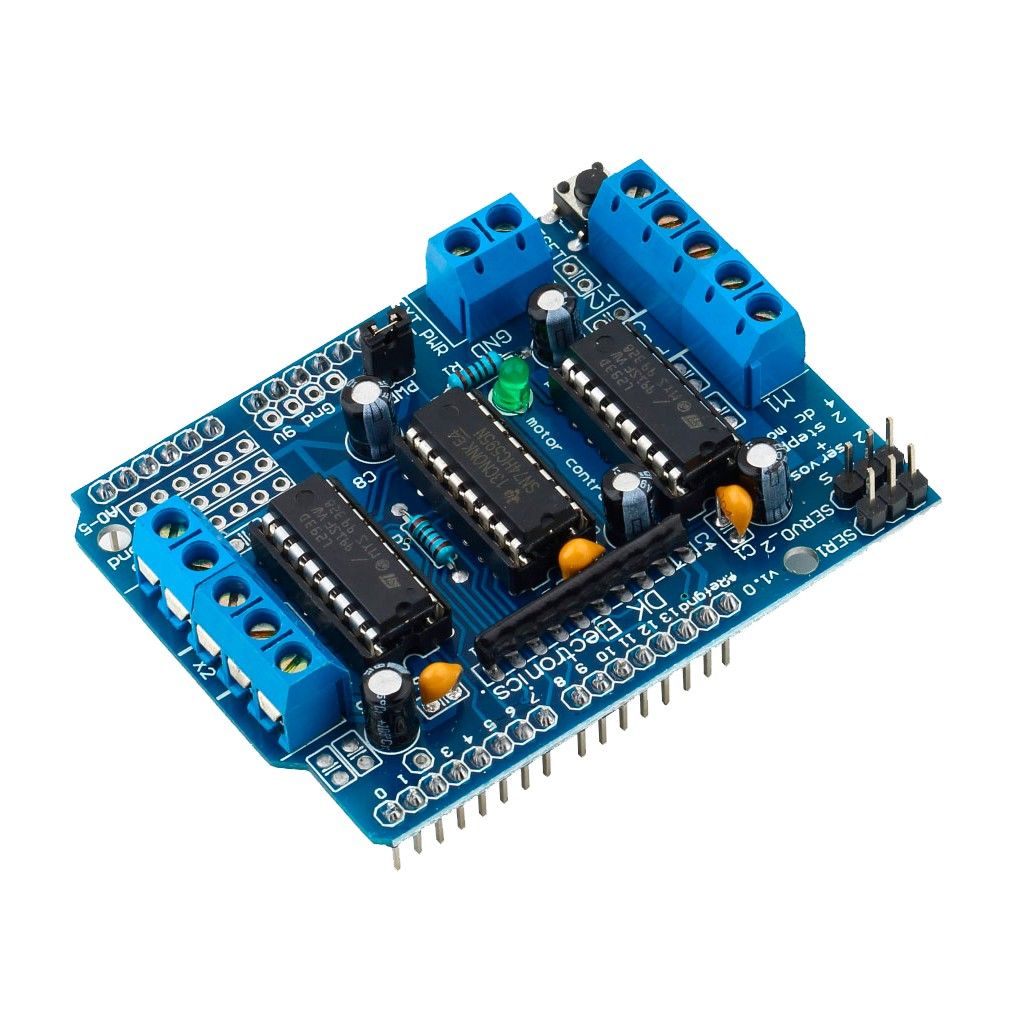
\includegraphics[width=3cm, height=2.3cm]{figures/04diseño_experimental/shield.jpg}    
    \\ \hline
    \textbf{4}  & Motor DC 12V con encoders    &  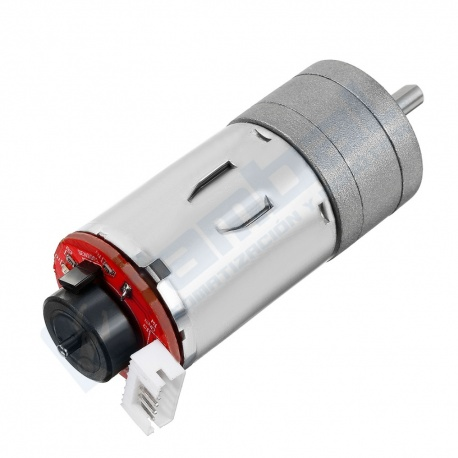
\includegraphics[width=3cm, height=2.3cm]{figures/04diseño_experimental/motor.jpg}    
    \\ \hline
    \textbf{5}  & LIDAR LD19       &   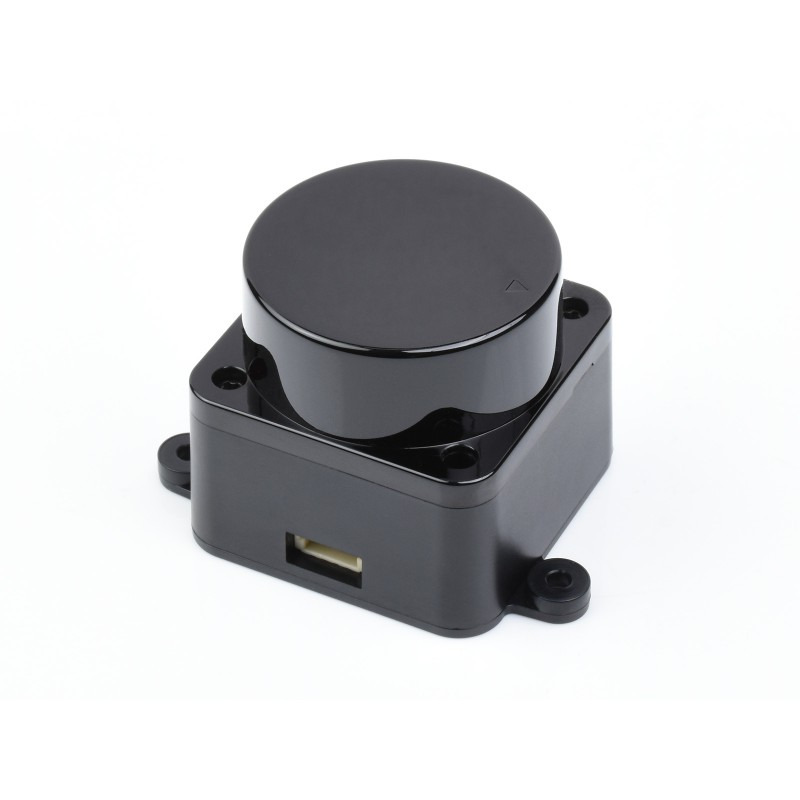
\includegraphics[width=3cm, height=2.3cm]{figures/04diseño_experimental/lidar.jpg}       \\ \hline
    \textbf{6}  & Orbbec Astra Pro &  
    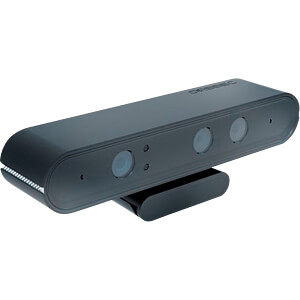
\includegraphics[width=3cm, height=2.3cm]{figures/04diseño_experimental/orbbec.jpg} 
    \\ \hline
    \textbf{7}  & Batería 11.1V    & 
    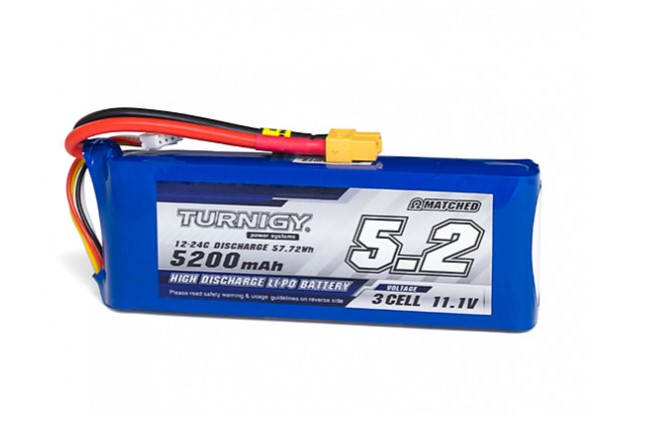
\includegraphics[width=3cm, height=2.3cm]{figures/04diseño_experimental/batería.jpg} 
    \\ \hline
    \textbf{8}  & Wit Motion BWT901BLECL    & 
    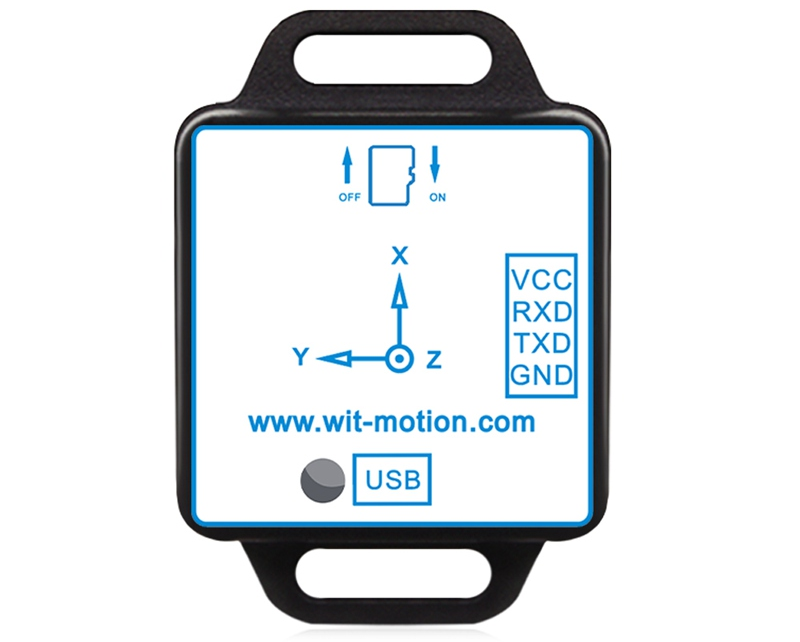
\includegraphics[width=3cm, height=2.3cm]{figures/04diseño_experimental/wit_motion.png} 
    \\ \hline
    \end{tabular}
    \caption{Componentes electrónicos} Fuente: Fabricación propia
\label{tab:componentes_electronicos}
\end{table}

\subsubsection{MODELO MATEMÁTICO}
La creación de un modelo matemático es esencial para la odometría de un robot \footnote{La odometría corresponde a la estimación de la posición de un robot durante la navegación apoyado por la información de diversos sensores}. La odometría se utiliza para estimar la posición de un robot en el corto plazo, ya que bastante susceptible a diversos errores, como lo son:
\begin{itemize}
    \item Los diámetros de las ruedas no son iguales.
    \item Alineamiento de las ruedas no es el mismo.
    \item Los encoders que se utilizan tienen errores asociados.
    \item Suelos desnivelados o resbaladizos.
\end{itemize}
En esta línea, es por ello que la odometría solo se utiliza para apoyar la labor del LIDAR y de la cámara de profundidad a largo plazo, sin embargo, es esencial en el corto plazo para estimar de manera correcta la posición. 

\begin{figure}[H]
\centering
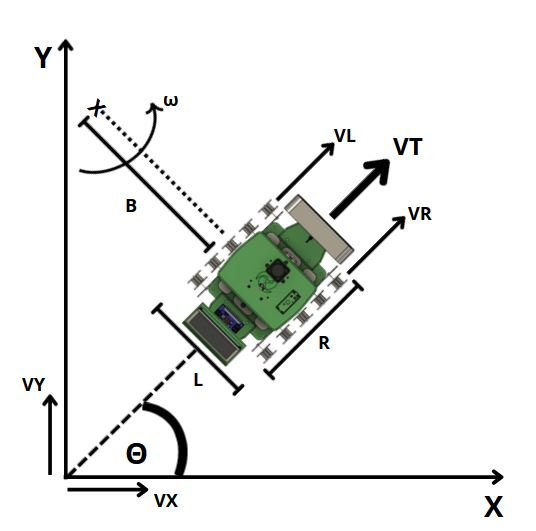
\includegraphics[width=15cm]{figures/04diseño_experimental/odometría.JPG}
\caption{Modelo matemático del robot diferencial utilizado en la memoria}
Fuente: Fabricación propia
\label{fig:robocop_odometría}
\end{figure}
Por lo tanto, para utilizar la odometría, es necesario realizar el modelo matemático, el cual se puede observar en la Figura \ref{fig:robocop_odometría}. A partir de dicha figura, se pueden definir las siguientes variables:
\begin{itemize}
    \item \textbf{$\omega$}: Representa la velocidad angular del robot, medido en $\frac{radianes}{segundos}$.
    \item \textbf{$X$}: Centro de giro.
    \item \textbf{$B$}: Radio de giro del robot, medido en $metros$.
    \item \textbf{$V_{R}$}: Velocidad de la rueda derecha, medido en $\frac{metros}{segundos}$.
    \item \textbf{$V_{L}$}: Velocidad de la rueda izquierda, medido en $\frac{metros}{segundos}$.
    \item \textbf{$V_{T}$}: Velocidad promedio, medido en $\frac{metros}{segundos}$
    \item \textbf{$L$}: Ancho del robot, medido en $metros$.
    \item \textbf{$R$}: Largo del robot, medido en $metros$.
    \item \textbf{$\theta$}: Representa el ángulo de giro del robot, medido en $radianes$.
    \item \textbf{$V_x$}: Velocidad en el eje x, medido en $\frac{metros}{segundos}$.
    \item \textbf{$V_y$}: Velocidad en el eje y, medido en $\frac{metros}{segundos}$.
\end{itemize}

El caso general, es decir, cuando el robot no se encuentra paralelo al eje X y al eje Y, las velocidad en  los ejes cartesianos se definen de la siguiente manera:
\[
V_X = V_T \cdot \cos{\theta}
\]
\[
V_Y = V_T \cdot \sin{\theta}
\]
Luego, al ser un robot diferencial, el giro viene dado por la diferencia entre las velocidad, es decir,
\[
V_L = \omega \cdot B
\]
\[
V_R = \omega \cdot (B + L)
\]
\[
\omega = \frac{V_R - V_L}{2}
\]

Por lo que el modelo matemático viene dado por:
\begin{equation}
    \dot{x} = \frac{V_R - V_L}{2} \cdot \cos{\theta}
    \label{ecuacion_1}
\end{equation}

\begin{equation}
    \dot{y} = \frac{V_R - V_L}{2} \cdot \sin{\theta}
    \label{ecuacion_2}
\end{equation}

\begin{equation}
    \dot{\omega} = \frac{V_R - V_L}{2}
    \label{ecuacion_3}
\end{equation}

Luego dichas ecuaciones, se utilizan para obtener la odometría y así publicar en el tópico ``/odom" la información correspondiente, es decir, la posición en eje Y, en el eje X y la orientación en el eje Z.



\subsubsection{DIAGRAMA DE FLUJO DE COMANDOS}
Con respecto al flujo de comandos, durante la memoria se consideraron dos ambientes. El primer ambiente, el cual es dónde el computador presente del robot procesa toda la información, se realizan los cálculos correspondientes, se envían las señales y reciben los datos de los sensores, entre otras acciones y por otra parte, se encuentra el segundo ambiente, el cual corresponde al microcontrolador y las tareas que este realiza como lo son el envió de las instrucciones a los motores, el envió de la información por parte de estos al computador y el procesamiento de las instrucciones provenientes desde el computador. 
El flujo de comandos se puede observar en detalle en la Figura \ref{fig:flujo_comandos}, en donde en primera instancia se observa que el robot se puede controlar de manera inalámbrica mediante un control de radio frecuencia o un control bluetooth (ya sea para largas distancia o cortas distancias respectivamente), a través del tópico \textbf{rc\_data}, el cual envía los datos obtenidos del control al computador, en este caso, una Orange Pi, esta última procesa los comandos recibidos, los mapea a las instrucciones correspondientes y los envía al microcontrolador Arduino a través de paquetes TCP mediante ros\_serial\footnote{ros\_serial provee de un protocolo de comunicación que tiene ROS, basado en el protocolo TCP, para comunicarse con diversos dispositivos y de esta manera enviar los mensajes de manera rápida y eficaz.}.

A su vez, la Orange Pi, debe procesar los datos recibidos tantos del LIDAR (enviados mediante el tópico de comunicación \textbf{scan}), los datos enviados desde la cámara 3D (enviados mediante el tópico de comunicación \textbf{raw\_image}) y con estos datos, construir los mapas bidimensionales y tridimensionales del entorno con los algoritmos de mapeo mencionados anteriormente.

Por otro lado, la Orange Pi también tiene como objetivo procesar los datos del LIDAR (utilizando el mismo tópico de comunicación nombrado anteriormente), los datos enviados por el sensor Wit Motion (enviados mediante el tópico de comunicación \textbf{imu}) y también, los datos enviados por el Arduino (enviados mediante el tópico \textbf{odometry}
), y así, una vez procesados estimar la posición del robot a través de los algoritmos de localización nombrados anteriormente.

Por último, el microcontrolador tiene como objetivo ser un canal de comunicación entre la orange pi y los motores, es decir, debe traducir los comandos enviados por el protocolo ros\_serial a instrucciones con los datos correspondientes para mover los motores con la velocidad y dirección correctos (enviados mediante el tópico \textbf{cmd\_vel}). También, el microcontrolador, debe recibir los datos de los encoders (enviados a través de los tópicos \textbf{left\_tick} y \textbf{right\_tick}, según el motor que corresponda), procesarlos y publicarlos mediante el tópico \textbf{odometry} para ser obtenidos y procesados en tiempo real por la Orange Pi.

\begin{figure}[H]
\centering
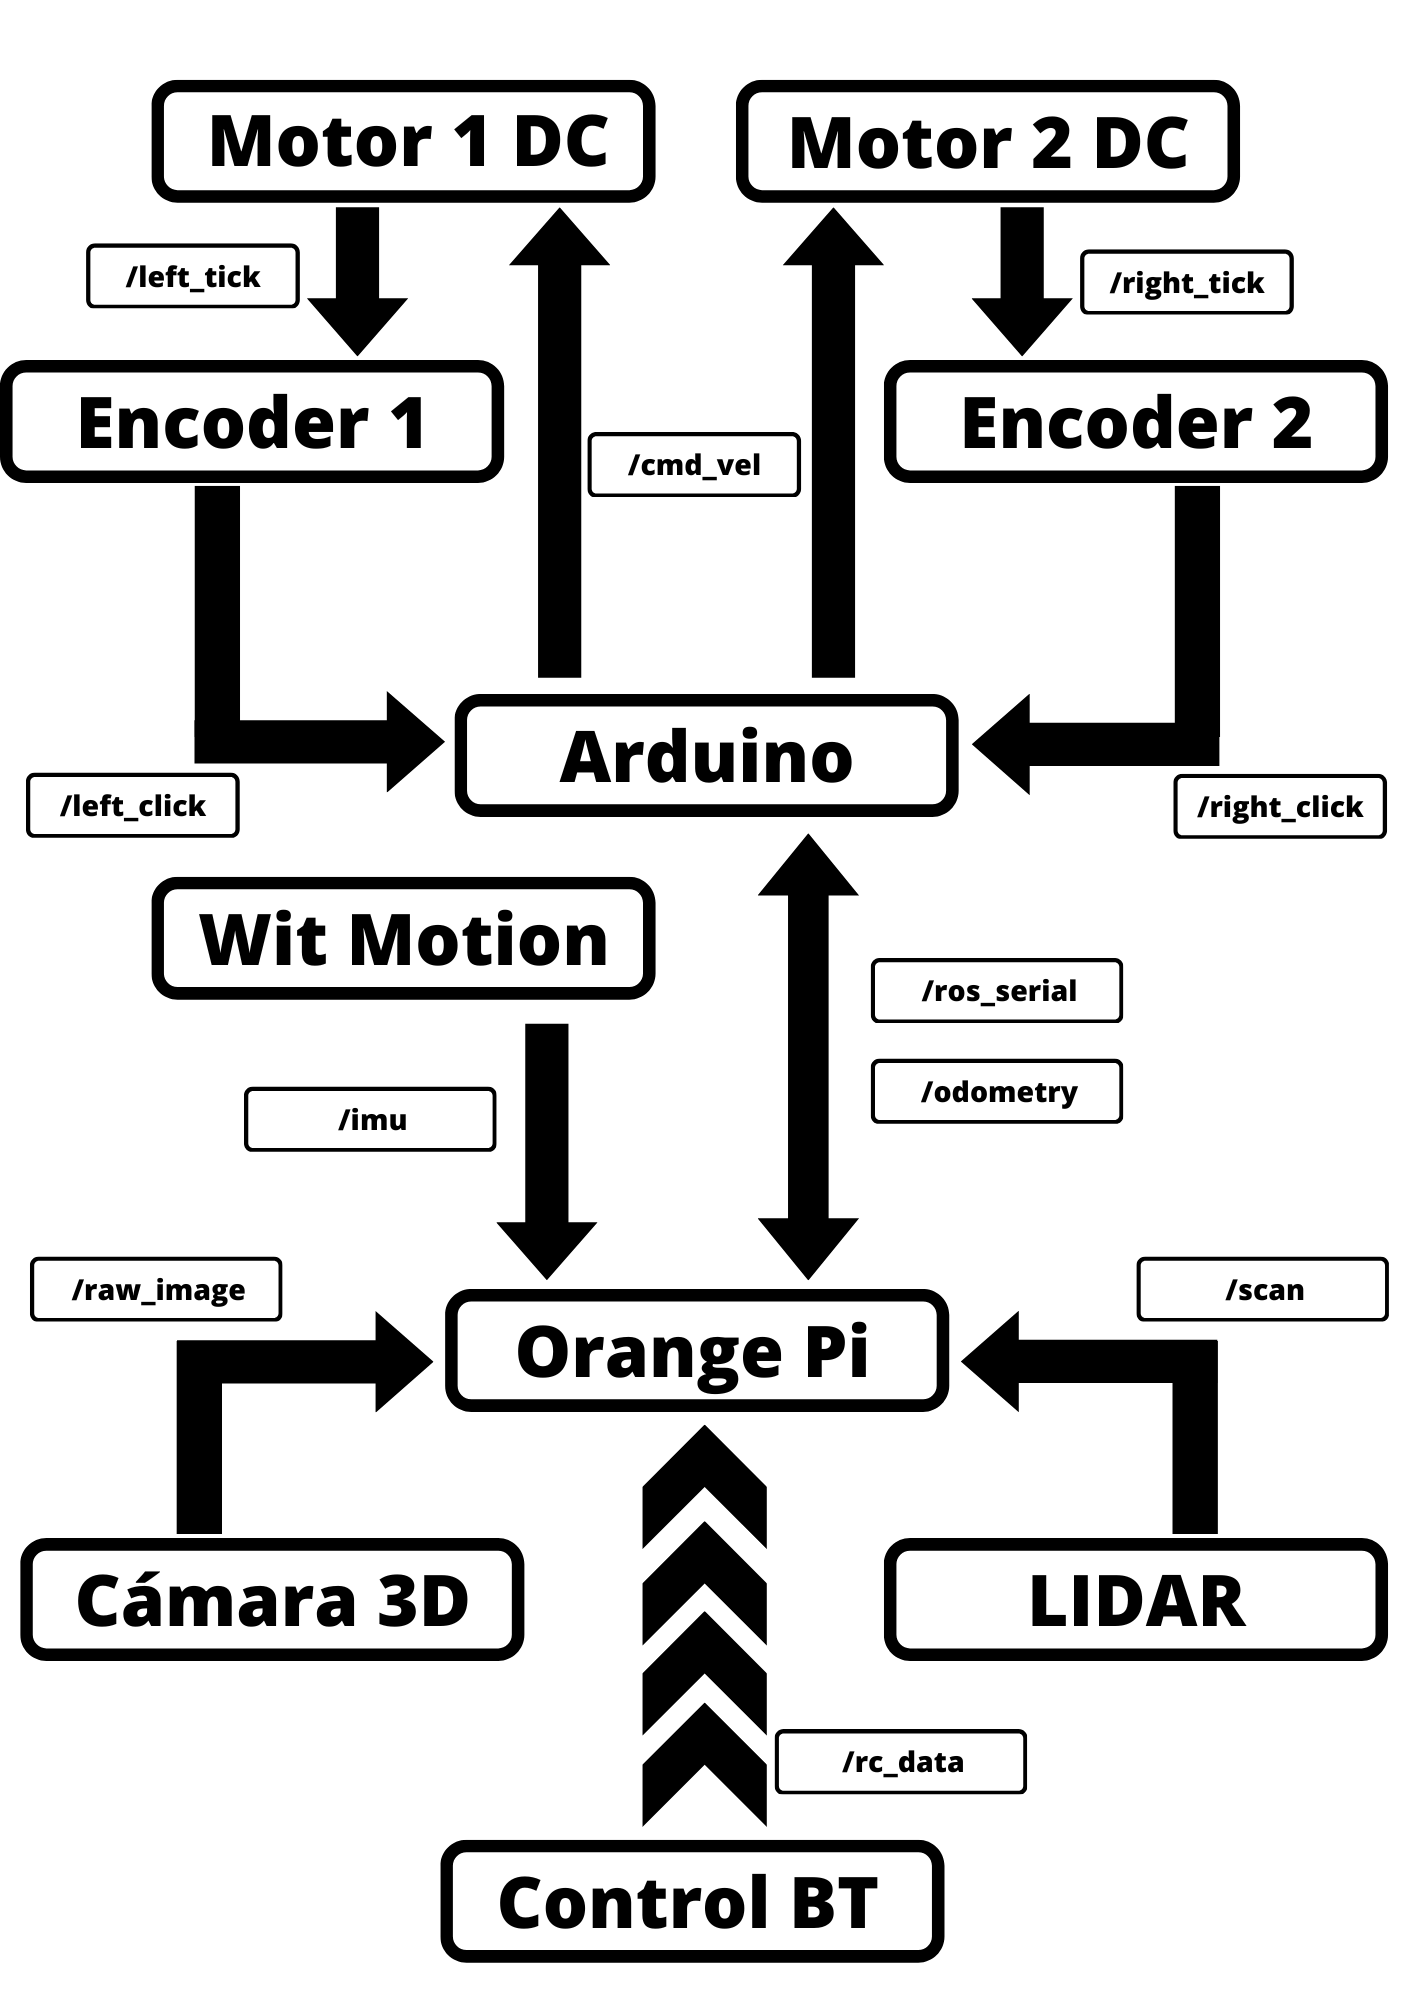
\includegraphics[width=10cm]{figures/04diseño_experimental/Flujo de comandos.png}
\caption{\label{fig:flujo_comandos} Flujo de los comandos e instrucciones} Fuente: Fabricación propia
\end{figure}



\subsubsection{PAQUETES DE ROS UTILIZADOS}
\begin{itemize}
    \item \textbf{ROS\_SERIAL:} Paquete utilizado para la comunicación entre la orange pi y el arduino, permite la utilización del protocolo de ROS, como también diversas librerías para optimizar el paso de mensajes.
    \item \textbf{DS4\_JOYSTICK:} Paquete utilizado para mapear los joystick, botones y giroscopios del control de la Play Station 4, de esta manera tener un control más cómodo sobre el robot.
    \item \textbf{LIDAR\_STL\_ROS:} Paquete que permite la comunicación entre la orange pi y el lidar, como también provee de librerías para utilizar los datos del LIDAR y de esta manera identificar distancias, obstáculos y la propia orientación del robot.
    \item \textbf{GAZEBO\_ROS:} Paquete que proporciona el entorno de simulación Gazebo, el cual, provee de herramientas de simulación, análisis de fuerzas físicas, como también permite modelar sensores como lo son los lidares y las cámaras de profundidad.
    \item \textbf{RVIZ\_ROS:} Paquete que provee el entorno de simulación RVIZ, el cual permite visualizar los datos provenientes de los diversos sensores utilizados en tiempo real, lo que a su vez, permite al usuario observar lo que está ocurriendo y como el robot está interpretando los datos. Provee de librerías para visualizar los datos del lidar, los datos de la cámara, generar nubes de puntos, entre otros elementos más.
    \item \textbf{MOVE\_BASE:} Paquete que proporciona los elementos básicos para identificar posiciones en el entorno de visualización RVIZ y provee la vinculación entre el planificadores global \footnote{El planificador global es aquel que construye la ruta entre la posición del robot y la posición final que se requiere alcanzar.}, el planificador local \footnote{El planificador local es aquel que en base a la ruta generada por el planificador global y el mapa de costes, produce los comandos de velocidad para mover el robot según la ruta indicada.} y el propio robot.
    \item \textbf{USB\_CAM:} Paquete que permite interactuar con las cámaras USB y provee de las librerías necesarias para utilizar las cámaras de profundidad con todas sus funciones, es decir, obtener las imágenes, comprimirlas, obtener los datos del lidar que contienen, transformar dichos datos a nubes de puntos, entre otras funcionalidades.
    \item \textbf{IMAGE\_VIEW:} Paquete que provee, en conjunto con el paquete anteriormente descrito, las librerías básicas para visualizar las imágenes obtenidas por las cámaras, el cual está optimizado para las cámaras de profundidad. A su vez, permite a través de sus librerías el envío de imágenes vía inalámbrica a la estación de control.
    \item \textbf{JOINT\_STATE\_PUBLISHER:} Paquete que proporciona librerías para establecer y publicar los estados de las uniones y así, permitir construir el modelo del robot tanto en Gazebo como en RVIZ a través de los archivos URDF, además provee de extensiones para integrar los sensores, cámaras y otros elementos en conjunto con el robot \footnote{URDF sigue un formato de archivo XML, el cual permite representar el modelo del robot}.
    \item \textbf{ROBOT\_STATE\_PUBLISHER:} Paquete que provee de las librerías necesarias para publicar el estado del robot al tópico tf, de esta manera, los componentes quedan disponibles para ser utilizados por cualquier otro elemento que se suscriba a dicho tópico. También permite modificar las posiciones y orientaciones de dichos elementos a través de las transformaciones correspondientes.
    \item \textbf{FRAME\_TRANSFORMATION:} El paquete proporciona las librerías necesarias para realizar un seguimiento a las coordenadas de los distintos componentes del robot, esto se realiza mediante transformaciones entre los distintos elementos, estructuras y sobretodo, marcos del robot y el ambiente.
    \item \textbf{CAMERA\_CALIBRATION:} El paquete permite realizar las calibraciones a las distintas cámaras existentes en el mercado, para así obtener las distorsiones correspondientes.
\end{itemize}

\subsubsection{MARCOS DE REFERENCIA}
Uno de los elementos esenciales para la navegación y localización, son los marcos de referencia, es decir, como el robot entiende el entorno y su posición en este a través de las coordenadas y orientaciones. En esta línea, cuando un robot se encuentra en el ambiente puede tener diversos marcos de referencia (generalmente se tiene un marco de referencia por cada componente), de esta manera es más sencillo tener control sobre el robot.
El robot sabe su posición en todo momento, sin embargo, dicha posición puede ser medida desde los diversos marcos de referencia y lo mismo ocurre con los obstáculos y objetos en el ambiente como se observa en la Figura \ref{fig:frames_explication}, es por ello, que se requieren transformaciones las cuales pueden ser traslaciones y rotaciones entre los diversos marcos de referencia.
\begin{figure}[H]
\centering
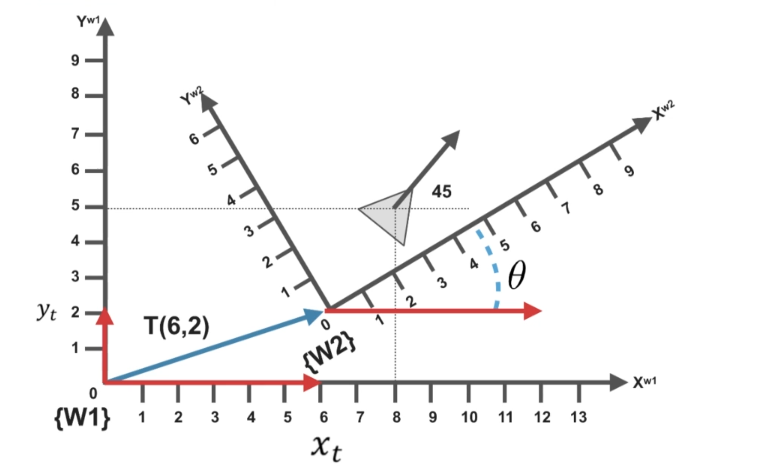
\includegraphics[width=15cm]{figures/04diseño_experimental/frames.png}
\caption{\label{fig:frames_explication} Transformación entre los marcos de referencia} Fuente: \cite{anis_koubaa_robot_2016}
\end{figure}
Con respecto a los marcos de referencia utilizados durante la memoria, estos se pueden observar en la Figura \ref{fig:frames_robocop} (construido con el comando \textbf{rqt\_graph}), donde se pueden identificar 5 niveles:
\begin{itemize}
    \item \textbf{Nivel 1:} Corresponde al nivel en dónde se encuentra el marco de referencia general, el cual tiene la información general sobre el ambiente, mostrado como \textbf{map}.
    \item \textbf{Nivel 2:} Corresponde al nivel en dónde está el marco de referencia conocido como odometría, el cual maneja la información del robot con respecto al mapa, mostrado como \textbf{odom}.
    \item \textbf{Nivel 3:} Corresponde al nivel dónde se encuentra el marco de referencia central del robot, mostrado como \textbf{base\_link}.
    \item \textbf{Nivel 4:} Corresponde al nivel dónde se encuentran los elementos del robot, se pueden observar los diversos componentes físicos como lo son los soportes y sensores.
    \item \textbf{Nivel 5:} Corresponde al último nivel en dónde se encuentran las ruedas y contienen la información con respecto a cada par de ruedas del robot desarrollado durante la memoria.
\end{itemize}

Con la información de los marcos de referencia y las transformaciones entre cada uno de ellos, el robot puede ubicarse en el mapa y planificar las rutas correspondientes ya que estas transformaciones también le permiten identificar las distancias a los obstáculos.

\begin{figure}[H]
\centering
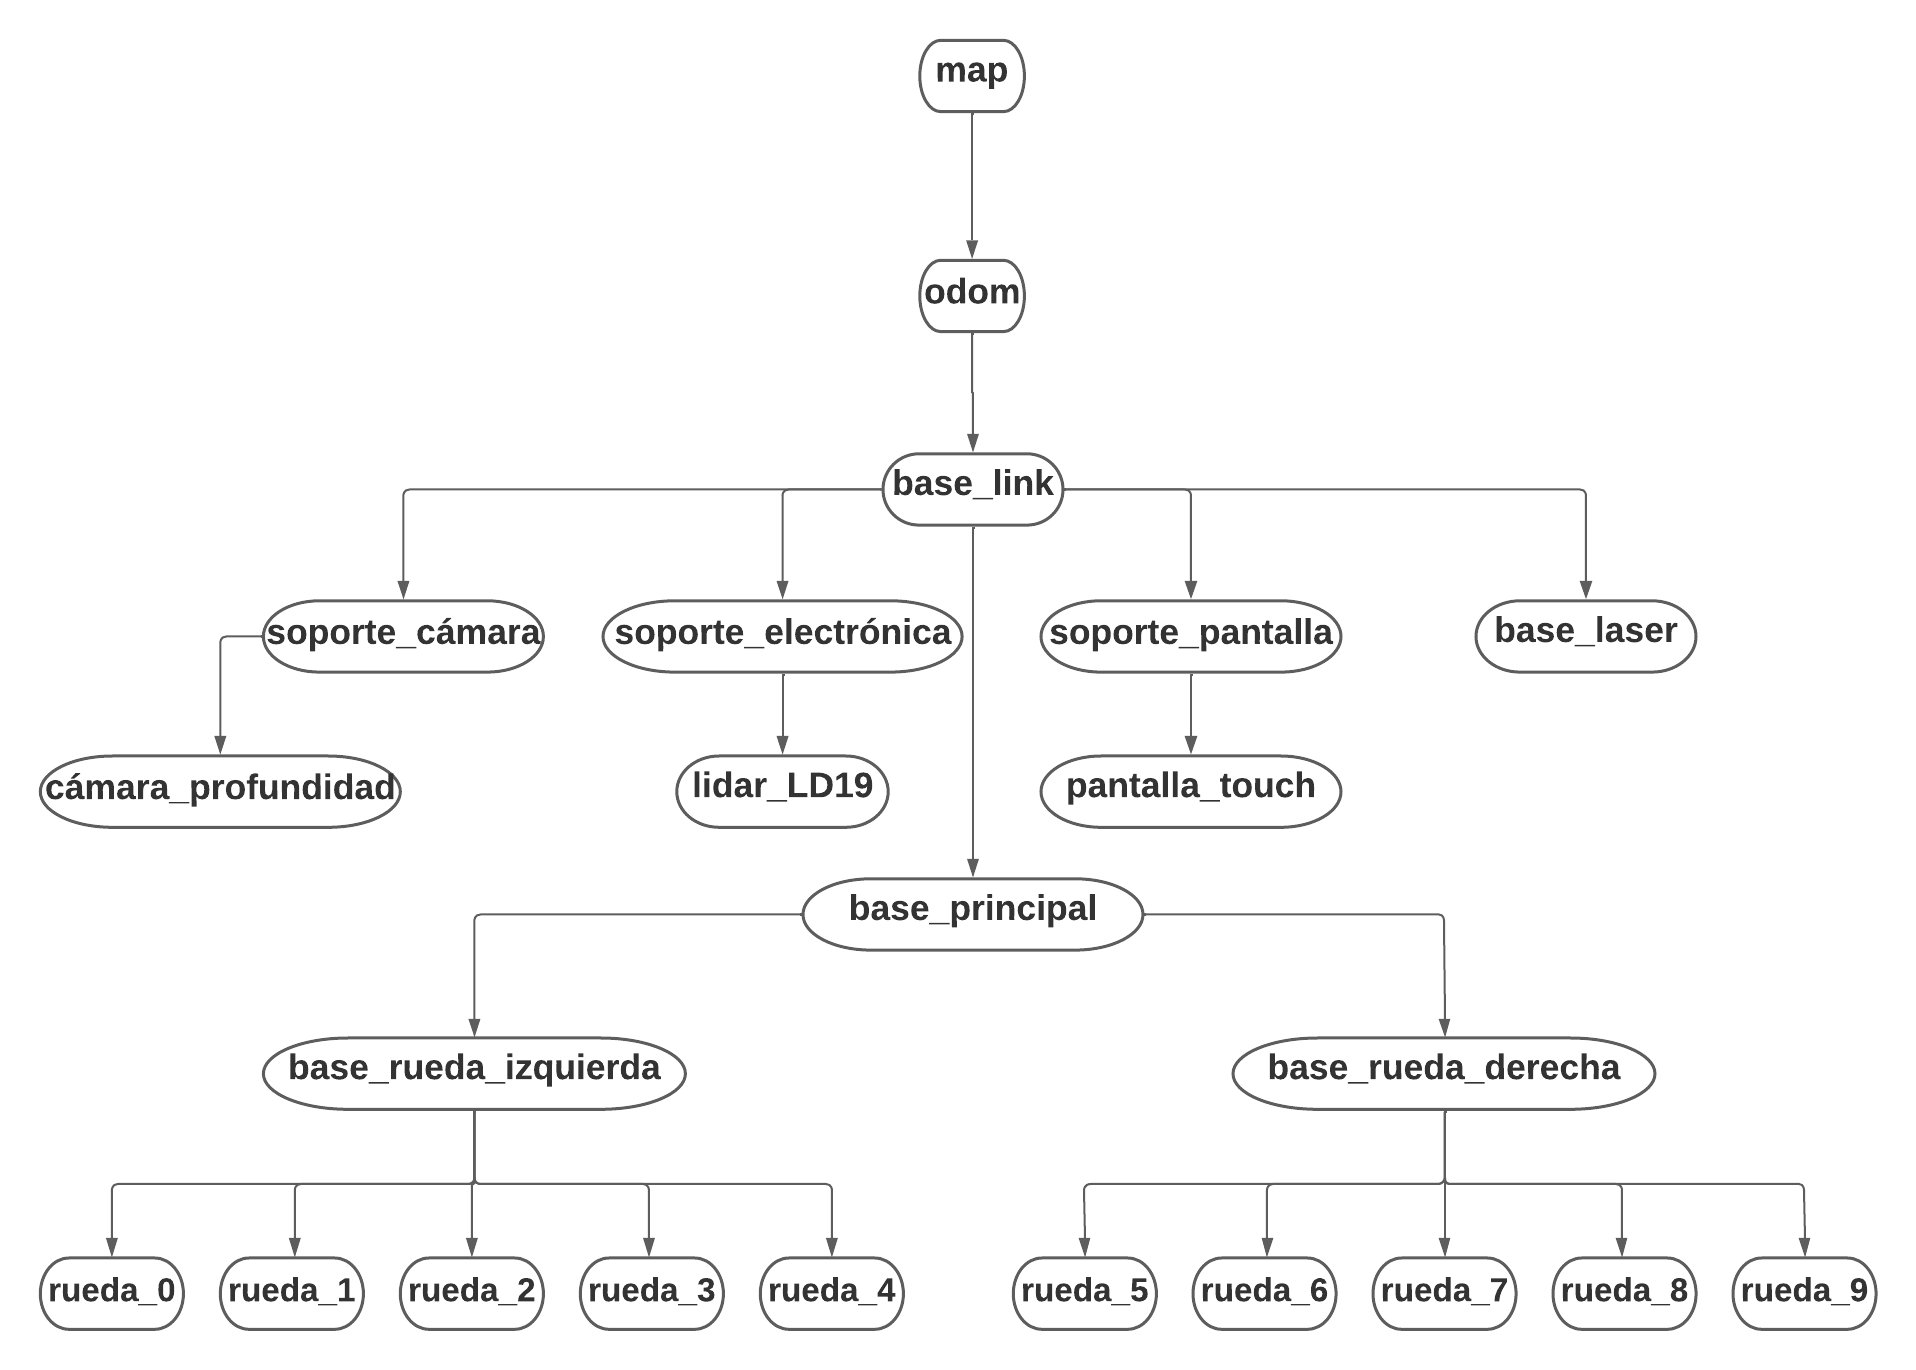
\includegraphics[width=18cm, height=11cm]{figures/04diseño_experimental/robocop_frames.png}
\caption{\label{fig:frames_robocop} Marcos de referencia utilizados para desarrollar la memoria} 
Fuente: Fabricación propia
\end{figure}

\newpage
\subsection{DEFINICIÓN DE LA EXPERIMENTACIÓN}
Con respecto a la experimentación, se utilizarán 5 ambientes reales los cuales contemplan una serie de desafíos en los que el robot debe completar a la cabalidad la tarea que se le asigne. En cada uno de los ambientes, se evaluará el desempeño del robot y sobretodo, de los algoritmos, en base a una serie de métricas que se especifican a continuación.

\subsubsection{MÉTRICAS DE DESEMPEÑO}
La evaluación del desempeño de los algoritmos se concentrará en 10 métricas las cuales se describen en la Tabla \ref{tab:metricas de evaluacion}. En dicha tabla se nombran las métricas a utilizar, como también las medidas con las cuales se evaluará dicho punto.

\begin{table}[H]
    \centering
    \begin{tabular}{|c|p{4cm}|c|p{8.5cm}|}
    \hline
    \textbf{N°} & \textbf{Nombre}             & \textbf{Medida} & \textbf{Descripción}                                                                               \\ \hline
    \textbf{1}  & Tiempo en generar el mapa   & Segundos        & Corresponde al tiempo en que tarda el algoritmo en construir el mapa.                              \\ \hline
    \textbf{2}  & Precisión del mapa generado & Porcentaje      & Corresponde a la diferencia porcentual entre el mapa real y el mapa generado.                      \\ \hline
    \textbf{3}  & Ruta planificada            & Metros          & Corresponde a la longitud de la ruta planificada entre la posición inicial y la posición final.    \\ \hline
    \textbf{4}  & Precisión de la ruta            & Porcentaje          & Corresponde a la diferencia porcentual entre la longitud de la ruta planificada y la ruta realizada.   
    \\ \hline
    \textbf{5}  & Tiempo en completar la ruta & Segundos        & Corresponde al tiempo en que se tarda en completar la ruta planificada.                            \\ \hline
    \textbf{6}  & Tiempo de localización      & Segundos        & Corresponde al tiempo en que tarda el algoritmo en localizar al robot dentro del mapa.             \\ \hline
    \textbf{7}  & Precisión de localización   & Porcentaje      & Corresponde a la diferencia porcentual entre la ubicación real y la ubicación estimada.            \\ \hline
    \textbf{8}  & Adaptación                  & Booleano        & Corresponde a la adaptación que tiene el algoritmo frente a los cambios en tiempo real del entorno \\ \hline
    \textbf{9}  & Consumo de memoria                  & Megabyte        & Corresponde al consumo de memoria que utiliza el algoritmo \\ \hline
    \textbf{10}  & Tamaño del archivo                 & Megabyte        & Corresponde tamaño del archivo del mapa generado por el algoritmo \\ \hline
    \end{tabular}
    \caption{Descripción de las métricas de evaluación}
    \label{tab:metricas de evaluacion}
\end{table}
Si bien existen más de una decena de métricas que se pueden utilizar para evaluar el desempeño del robot y de los algoritmos anteriormente descritos, que se utilizarán las 10 métricas nombradas dado que engloban el comportamiento general que debe tener todo algoritmo de mapeo, navegación y localización. 

\newpage
\subsection{DEFINICIÓN DE PRUEBAS}
La experimentación se realizó sobre 5 ambientes distintos, en los cuales no solo la disposición de los obstáculos cambió, sino también, la dificultad para la creación de los mapas, planeamiento de rutas y la propia movilización. Se eligieron estos 5 ambientes, ya que abarcan, en términos generales, todos los aspectos en los cuales un robot se puede desenvolver. Los aspectos específicos, imágenes y dimensiones se verán en las secciones correspondientes a cada ambiente. 

En términos generales, las pruebas consistirán en el movimiento del robot desde una posición inicial hasta una posición final, como se muestra en la Figura \ref{fig:ambientes_explicacion}, cada ambiente será distinto y tendrá características específicas que luego se nombrará. De esta manera, se evaluarán las métricas descritas en la Tabla \ref{tab:metricas de evaluacion}  a través del desempeño del robot durante dichas pruebas, también para evaluar el comportamiento del algoritmo se seleccionarán dos algoritmos correspondientes SLAM 3D y SLAM 2D, OctoMap Library y el algoritmo Hector Mapping respectivamente y así comparar el desempeño tanto tridimensional como bidimensional del algoritmo propuesto.

\begin{figure}[H]
\centering
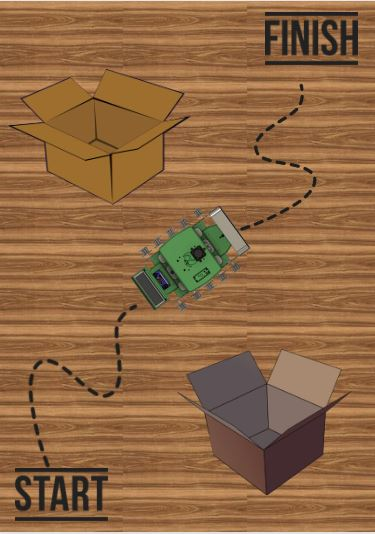
\includegraphics[width=7cm]{figures/04diseño_experimental/ambientes_explicacion.JPG}
\caption{\label{fig:ambientes_explicacion} Explicación general de las pruebas} 
Fuente: Fabricación propia
\end{figure}

\newpage
\subsubsection{DESCRIPCIÓN DEL AMBIENTE NÚMERO 1}
\textbf{Escala de dificultad - } 1/5:

\hspace{5mm} \textbf{Presenta Obstáculos:} No

\hspace{5mm} \textbf{Presenta Sub-Punto:} No

\hspace{5mm} \textbf{Presenta Zonas Prohibidas:} No

El primer ambiente donde se realizarán la prueba se puede observar en la Figura \ref{fig:ambiente_1}. Es un ambiente sencillo, sin obstáculos, el cual se asemeja al comportamiento del robot en espacios abiertos, sin obstáculos. Dicho ambiente consta de un área de prueba de aproximadamente 20 [$m^{2}$], en dónde se puede observar una \textbf{posición inicial} y una \textbf{posición final}.

En este ambiente, el robot tiene por objetivo en primera instancia mapear el entorno para generar el mapa de navegación, luego de generado el mapa, el robot debe planificar la ruta desde la posición inicial hasta la posición final y por último, el robot debe localizarse en todo momento dentro del mapa. Cómo se mencionó anteriormente, en este ambiente no existirán obstáculos, ni zonas prohibidas ni tampoco sub-puntos en la ruta \footnote{Llámese sub-puntos a aquellas paradas necesarias o requeridas durante la realización de las pruebas.}.

\begin{figure}[H]
    \centering
    \begin{subfigure}[b]{0.30\textwidth}
    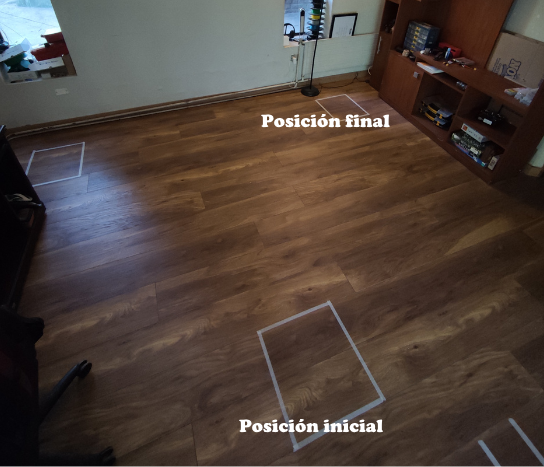
\includegraphics[width=\textwidth, height=\textwidth]{figures/04diseño_experimental/ambiente_1/ambiente_1_1.png}
    \caption{Vista lateral izquierda}
    \label{fig:ambiente_1_1}
    \end{subfigure}
    \begin{subfigure}[b]{0.30\textwidth}
    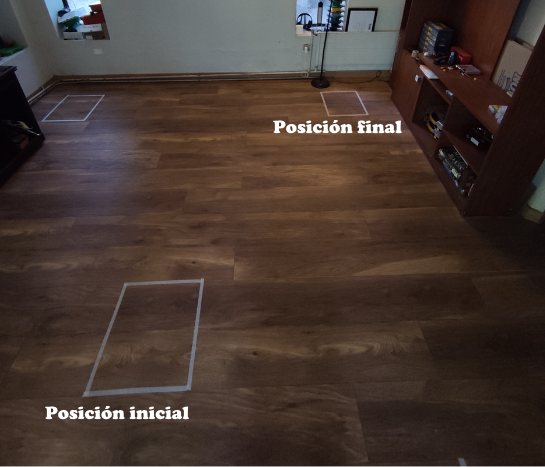
\includegraphics[width=\textwidth, height=\textwidth]{figures/04diseño_experimental/ambiente_1/ambiente_1_2.png}
    \caption{Vista central}
    \label{fig:ambiente_1_2}
    \end{subfigure}
    \begin{subfigure}[b]{0.30\textwidth}
    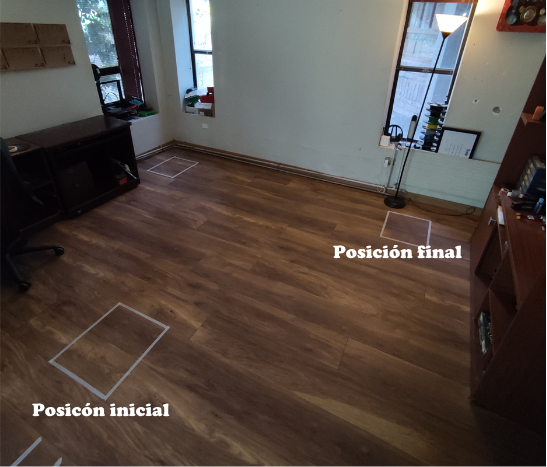
\includegraphics[width=\textwidth, height=\textwidth]{figures/04diseño_experimental/ambiente_1/ambiente_1_3.png}
    \caption{Vista lateral derecha}
    \label{fig:ambiente_1_3}
    \end{subfigure}
    \caption{Ambiente de pruebas número 1 }
    Fuente: Fabricación propia
    \label{fig:ambiente_1}
\end{figure} 

Cabe destacar, que el piso del ambiente 1 y de los demás ambientes, es de madera, ya que de esta manera se evitan problemas como que las ruedas derrapen, se tranquen o existan problemas de movimiento, esto no quiere decir que no existan problemas, sin embargo, de esta manera se minimizan dichos errores.

\newpage
\subsubsection{DESCRIPCIÓN DEL AMBIENTE NÚMERO 2}
\textbf{Escala de dificultad -} 2/5:

\hspace{5mm} \textbf{Presenta Obstáculos:} Si, único

\hspace{5mm} \textbf{Presenta Sub-Punto:} No

\hspace{5mm} \textbf{Presenta Zonas Prohibidas:} No

El segundo ambiente en donde se testearán los algoritmos, se pueden observar en la Figura \ref{fig:ambiente_2}. Dicho ambiente, cuenta con una \textbf{posición inicial} y una \textbf{posición final}, como también consta de un área de prueba de aproximadamente 20 [$m^{2}$] donde se asemeja a entornos con obstáculos ocasionales y fijos, en este sentido, en la imagen, se observan 2 obstáculos que se encuentran en contacto los cuales se describen a continuación:
\begin{itemize}
    \item \textbf{Obstáculo 1:} Una caja con un área basal de 0.6 [$m$] $\cdot$ 0.5 [$m$], es decir, 0.3 [$m^{2}$]. A una distancia de la posición inicial de aproximadamente 1.4 [$m$].
    \item \textbf{Obstáculo 2:} Una caja con un área basal de 0.4 [$m$] $\cdot$ 0.4 [$m$], es decir, 0.16 [$m^{2}$]. A una distancia de la posición inicial de aproximadamente 1.2 [$m$].
\end{itemize} 

\begin{figure}[H]
    \centering
    \begin{subfigure}[b]{0.30\textwidth}
    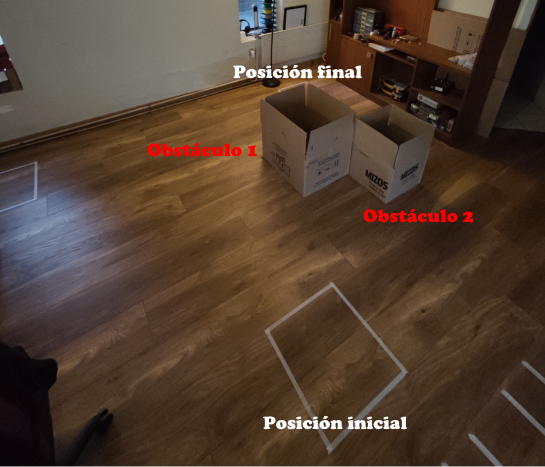
\includegraphics[width=\textwidth, height=\textwidth]{figures/04diseño_experimental/ambiente_2/ambiente_2_1.png}
    \caption{Vista lateral izquierda}
    \label{fig:ambiente_2_1}
    \end{subfigure}
    \begin{subfigure}[b]{0.30\textwidth}
    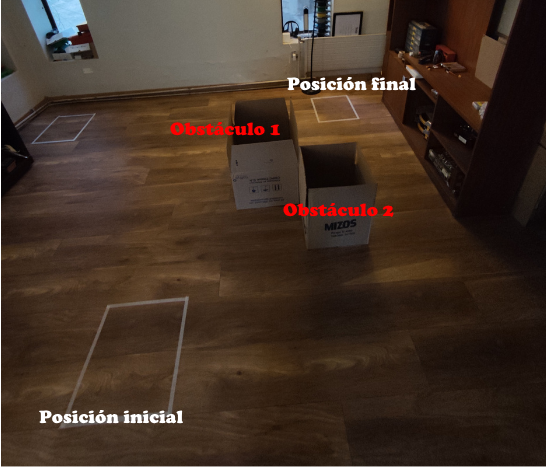
\includegraphics[width=\textwidth, height=\textwidth]{figures/04diseño_experimental/ambiente_2/ambiente_2_2.png}
    \caption{Vista central}
    \label{fig:ambiente_2_2}
    \end{subfigure}
    \begin{subfigure}[b]{0.30\textwidth}
    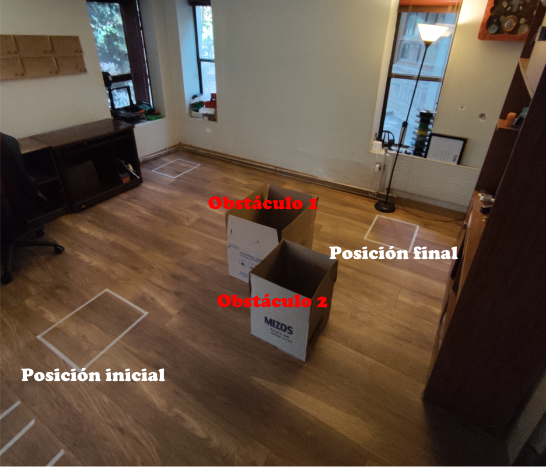
\includegraphics[width=\textwidth, height=\textwidth]{figures/04diseño_experimental/ambiente_2/ambiente_2_3.png}
    \caption{Vista lateral derecha}
    \label{fig:ambiente_2_3}
    \end{subfigure}
    \caption{Ambiente de pruebas número 2 }
    Fuente: Fabricación propia
    \label{fig:ambiente_2}
\end{figure} 

Al igual que en el ambiente número 1, el robot tiene por objetivo crear el mapa del entorno, esta vez, con los 2 obstáculos (aunque bien se podrían tomar como un solo gran obstáculo), luego realizar la planificación de la ruta desde la posición inicial, hasta la posición final, dónde no existen zonas prohibidas ni tampoco sub-puntos en la ruta y por último, localizarse en todo momento de la navegación. 

\newpage
\subsubsection{DESCRIPCIÓN DEL AMBIENTE NÚMERO 3}
\textbf{Escala de dificultad -} 3/5:

\hspace{5mm} \textbf{Presenta Obstáculos:} Si, múltiples

\hspace{5mm} \textbf{Presenta Sub-Punto:} No

\hspace{5mm} \textbf{Presenta Zonas Prohibidas:} No

El tercer ambiente en donde se testearán los algoritmos, se pueden observar en la Figura \ref{fig:ambiente_3}, Dicho ambiente, al igual que los anteriores, cuenta con una \textbf{posición inicial} y una \textbf{posición final}, en una zona de pruebas de aproximadamente 20 [$m^{2}$]. Este ambiente asemeja más al entorno real del día a día, ya que contempla la aparición de 3 obstáculos separados, los cuales que se definirán a continuación:

\begin{itemize}
    \item \textbf{Obstáculo 1:} Una caja con un área basal de 0.2 [$m$] $\cdot$ 0.2 [$m$], es decir, 0.04 [$m^{2}$]. A una distancia de la posición inicial de aproximadamente 2 [$m$].
    \item \textbf{Obstáculo 2:} Una caja con un área basal de 0.4 [$m$] $\cdot$ 0.4 [$m$], es decir, 0.16 [$m^{2}$]. A una distancia de la posición inicial de aproximadamente 1.2 [$m$].
    \item \textbf{Obstáculo 3:} Una caja con un área basal de 0.6 [$m$] $\cdot$ 0.5 [$m$], es decir, 0.3 [$m^{2}$]. A una distancia de la posición inicial de aproximadamente 1.4 [$m$].
\end{itemize} 

\begin{figure}[H]
    \centering
    \begin{subfigure}[b]{0.30\textwidth}
    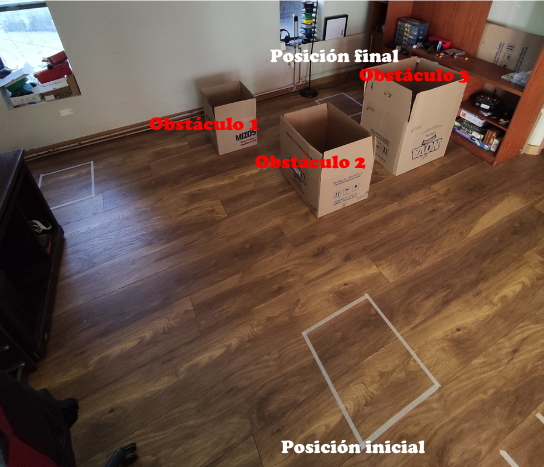
\includegraphics[width=\textwidth, height=\textwidth]{figures/04diseño_experimental/ambiente_3/ambiente_3_1.png}
    \caption{Vista lateral izquierda}
    \label{fig:ambiente_3_1}
    \end{subfigure}
    \begin{subfigure}[b]{0.30\textwidth}
    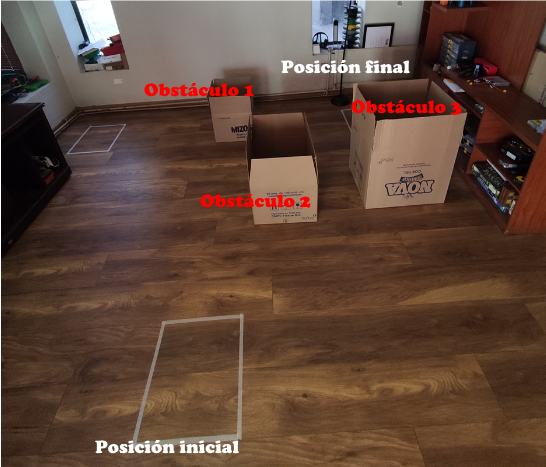
\includegraphics[width=\textwidth, height=\textwidth]{figures/04diseño_experimental/ambiente_3/ambiente_3_2.png}
    \caption{Vista central}
    \label{fig:ambiente_3_2}
    \end{subfigure}
    \begin{subfigure}[b]{0.30\textwidth}
    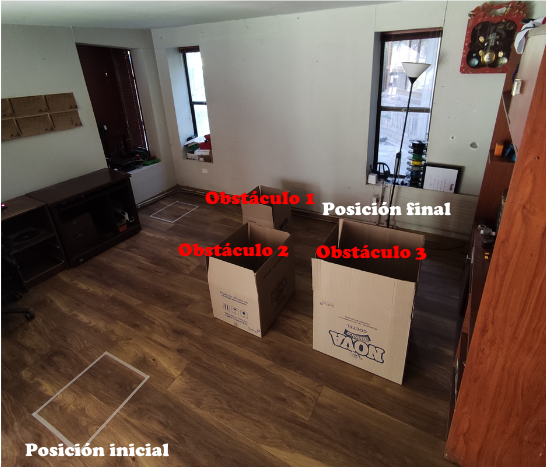
\includegraphics[width=\textwidth, height=\textwidth]{figures/04diseño_experimental/ambiente_3/ambiente_3_3.png}
    \caption{Vista lateral derecha}
    \label{fig:ambiente_3_3}
    \end{subfigure}
    \caption{Ambiente de pruebas número 3 }
    Fuente: Fabricación propia
    \label{fig:ambiente_3}
\end{figure}

En el ambiente número 3, el robot también tiene por objetivo crear el mapa del entorno, por lo que la disposición de los 3 obstáculos en destinas posiciones dificulta esta tarea, luego de realizada dicha tarea, el robot debe planificar la ruta desde la posición inicial hasta la posición final y también debe localizarse en todo momento. La diferencia con respecto al ambiente número 2, es que al estar los obstáculos separados tanto la navegación como el mapeo se dificultan más y también se asemejan más a entornos reales (al igual que en los 2 ambientes anteriores, no existen sub-puntos en la ruta, ni tampoco zonas prohibidas).

\subsubsection{DESCRIPCIÓN DEL AMBIENTE NÚMERO 4}
\textbf{Escala de dificultad -} 4/5:

\hspace{5mm} \textbf{Presenta Obstáculos:} Si, múltiples

\hspace{5mm} \textbf{Presenta Sub-Punto:} Si

\hspace{5mm} \textbf{Presenta Zonas Prohibidas:} No

El cuarto ambiente en donde se testearán los algoritmos, se pueden observar en la Figura \ref{fig:ambiente_4}. Dicho ambiente, al igual que los anteriores, cuenta con una \textbf{posición inicial} y una \textbf{posición final}, sin embargo, se agrega el \textbf{sub-punto A}. El ambiente asemeja a entornos donde el robot debe suplir tarea consecutivas, pero separadas espacialmente.
El entorno de pruebas es de aproximadamente 20 [$m^{2}$] y en este entorno, se pueden observar 4 obstáculos los cuales se describen a continuación:
\begin{itemize}
    \item \textbf{Obstáculo 1:} Una caja con un área basal de 0.4 [$m$] $\cdot$ 0.6 [$m$], es decir, 0.24 [$m^{2}$]. A una distancia de la posición inicial de aproximadamente 1 [$m$].
    \item \textbf{Obstáculo 2:} Una caja con un área basal de 0.2 [$m$] $\cdot$ 0.2 [$m$], es decir, 0.04 [$m^{2}$]. A una distancia de la posición inicial de aproximadamente 2 [$m$].
    \item \textbf{Obstáculo 3:} Una caja con un área basal de 0.4 [$m$] $\cdot$ 0.4 [$m$], es decir, 0.16 [$m^{2}$]. A una distancia de la posición inicial de aproximadamente 1.2 [$m$].
    \item \textbf{Obstáculo 4:} Una caja con un área basal de 0.6 [$m$] $\cdot$ 0.5 [$m$], es decir, 0.3 [$m^{2}$]. A una distancia de la posición inicial de aproximadamente 1.4 [$m$].
\end{itemize} 

\begin{figure}[H]
    \centering
    \begin{subfigure}[b]{0.30\textwidth}
    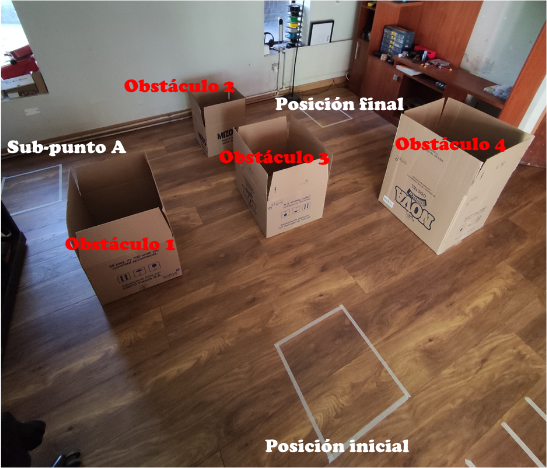
\includegraphics[width=\textwidth, height=\textwidth]{figures/04diseño_experimental/ambiente_4/ambiente_4_1.png}
    \caption{Vista lateral izquierda}
    \label{fig:ambiente_4_1}
    \end{subfigure}
    \begin{subfigure}[b]{0.30\textwidth}
    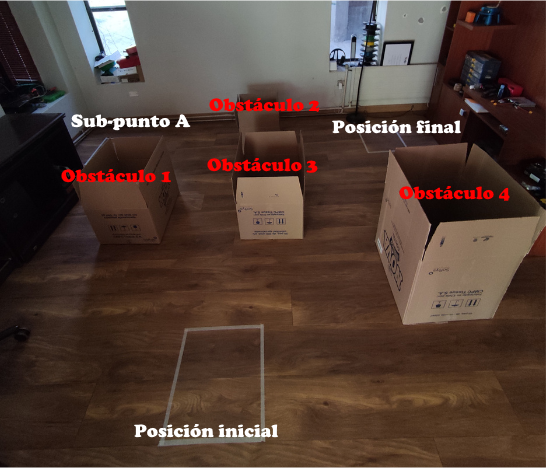
\includegraphics[width=\textwidth, height=\textwidth]{figures/04diseño_experimental/ambiente_4/ambiente_4_2.png}
    \caption{Vista central}
    \label{fig:ambiente_4_2}
    \end{subfigure}
    \begin{subfigure}[b]{0.30\textwidth}
    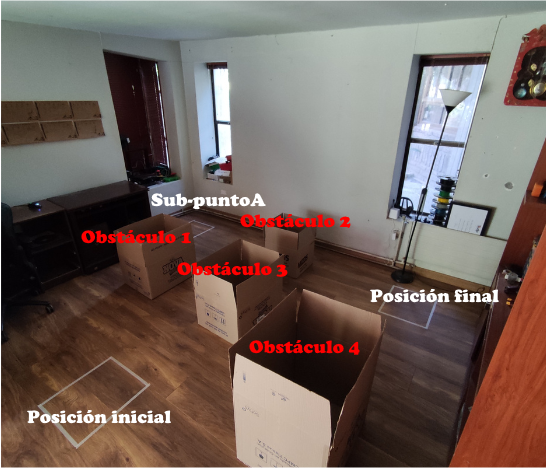
\includegraphics[width=\textwidth, height=\textwidth]{figures/04diseño_experimental/ambiente_4/ambiente_4_3.png}
    \caption{Vista lateral derecha}
    \label{fig:ambiente_4_3}
    \end{subfigure}
    \caption{Ambiente de pruebas número 4 }
    Fuente: Fabricación propia
    \label{fig:ambiente_4}
\end{figure}

En el ambiente número 4, el robot tiene por objetivo nuevamente mapear el entorno y así generar el mapa que le servirá para navegar. A diferencia de los ambientes testeados anteriormente, se le añade un nivel extra de dificultad al agregar un sub-punto en la ruta, es decir, el robot luego de mapear debe planificar la ruta para ir desde la posición inicial, hasta el sub-punto A y luego ir desde el sub-punto A hasta la posición final, dónde también el robot de ser capaz de localizarse en todo momento.

\subsubsection{DESCRIPCIÓN DEL AMBIENTE NÚMERO 5}
\textbf{Escala de dificultad: -} 5/5:

\hspace{5mm}  \textbf{Presenta Obstáculos:} Si, múltiples

\hspace{5mm}  \textbf{Presenta Sub-Punto:} Si

\hspace{5mm}  \textbf{Presenta Zonas Prohibidas:} Si

Por último, el quinto ambiente en donde se testearán los algoritmos, se pueden observar en la Figura \ref{fig:ambiente_5}. Dicho ambiente, al igual que el ambiente número 4, cuenta con una \textbf{posición inicial}, una \textbf{posición final} y un \textbf{sub-punto A}, sin embargo, aparecen 2 zonas prohibidas \footnote{Una zona prohibida, se entenderá como una zona bidimensional, en dónde está prohibido su paso, sin embargo, no existe una estructura que define su área. En caso de que el robot toque dicha zona se le agregará un 10\% de penalización a la ruta planificada y al tiempo en completar la ruta.}, las cuales se describirán más adelante. El ambiente, asemeja a un escenario completo, es decir, se encuentran todos los elementos posibles que pueden afectar el desplazamiento del robot y a los cuales los algoritmos se deben adaptar. El entorno de pruebas continua siendo de aproximadamente 20 [$m^{2}$] y en este entorno, se pueden observar 3 obstáculos y 2 zonas prohibidas, los cuales se describen a continuación:
\begin{itemize}
    \item \textbf{Obstáculo 1:} Una caja con un área basal de 0.4 [$m$] $\cdot$ 0.6 [$m$], es decir, 0.24 [$m^{2}$]. A una distancia de la posición inicial de aproximadamente 1 [$m$].
    \item \textbf{Obstáculo 2:} Una caja con un área basal de 0.2 [$m$] $\cdot$ 0.2 [$m$], es decir, 0.04 [$m^{2}$]. A una distancia de la posición inicial de aproximadamente 2 [$m$].
    \item \textbf{Obstáculo 3:} Una caja con un área basal de 0.4 [$m$] $\cdot$ 0.4 [$m$], es decir, 0.16 [$m^{2}$]. A una distancia de la posición inicial de aproximadamente 1.2 [$m$].
    \item \textbf{Zona prohibida 1:} Una caja con un área basal de 0.3 [$m$] $\cdot$ 0.4 [$m$], es decir, 0.12 [$m^{2}$]. A una distancia de la posición inicial de aproximadamente 0.8 [$m$].
    \item \textbf{Zona prohibida 2:} Una caja con un área basal de 0.3 [$m$] $\cdot$ 0.3 [$m$], es decir, 0.09 [$m^{2}$]. A una distancia de la posición inicial de aproximadamente 1. [$m$].
\end{itemize} 

\begin{figure}[H]
    \centering
    \begin{subfigure}[b]{0.30\textwidth}
    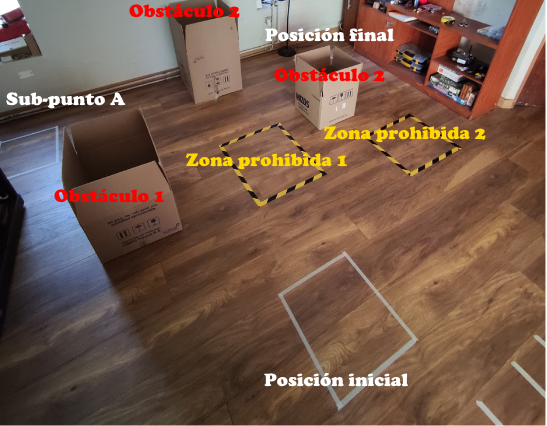
\includegraphics[width=\textwidth, height=\textwidth]{figures/04diseño_experimental/ambiente_5/ambiente_5_1.png}
    \caption{Vista lateral izquierda}
    \label{fig:ambiente_5_1}
    \end{subfigure}
    \begin{subfigure}[b]{0.30\textwidth}
    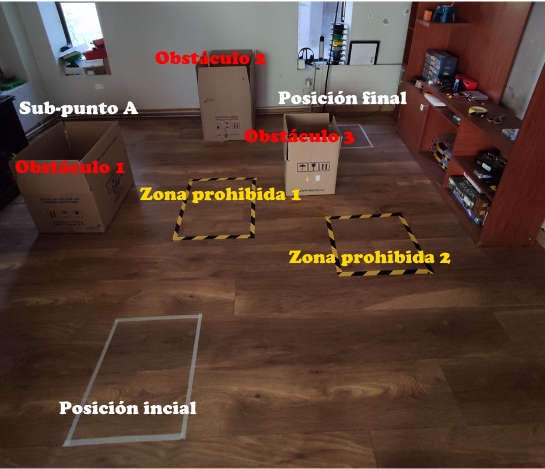
\includegraphics[width=\textwidth, height=\textwidth]{figures/04diseño_experimental/ambiente_5/ambiente_5_2.png}
    \caption{Vista central}
    \label{fig:ambiente_5_2}
    \end{subfigure}
    \begin{subfigure}[b]{0.30\textwidth}
    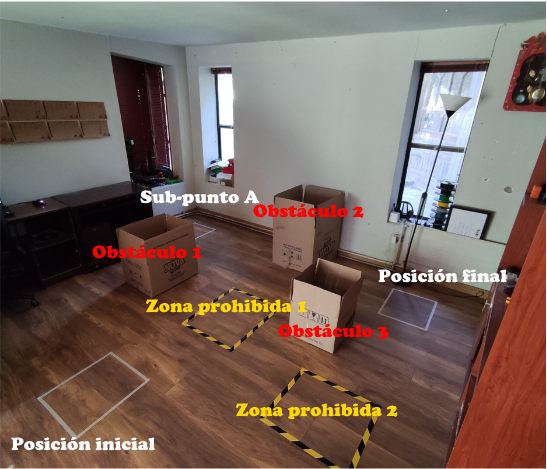
\includegraphics[width=\textwidth, height=\textwidth]{figures/04diseño_experimental/ambiente_5/ambiente_5_3.png}
    \caption{Vista lateral derecha}
    \label{fig:ambiente_5_3}
    \end{subfigure}
    \caption{Ambiente de pruebas número 5 }
    Fuente: Fabricación propia
    \label{fig:ambiente_5}
\end{figure}

En este último ambiente, el robot tiene por objetivo además de mapear el entorno completamente, planificar la ruta desde la posición inicial hasta el Sub-punto A y luego desde dicho punto hasta la posición final, localizarse en todo momento, pero al agregar zonas prohibidas el desplazamiento queda restringido y los algoritmo se deben adaptar a dicha circunstancia y no pueden transitar por el lugar pese a no existir un obstáculo definido.

